\subsection{Material properties}

The nessesary Cherenkov properties of materials include refraction index and absorption lenght for a range of photon energies (see \texttt{hdds/Material{\_}HDDS.xml}). The materials coupling together the elements of the detector optical system can introduce additional photon losses due to their poor Cherenkov properties. 

The following table summarizes the sources for the material properties used in the simulation. The refraction index data was taken from (or compared to) (*) \\ \url{https://refractiveindex.info}. 

\vspace{0.5cm}
\begin{tabular}{| c | c | c |}
\hline
\textit{material} & \textit{refraction index} & \textit{absorption length} \\
\hline
Fused Silica & * & \cite{Epotek} \\
\hline
Water & * and~\cite{EpotekData} & based on~\cite{water} and~\cite{water2} \\
\hline
Epotek 301-2 & \cite{EpotekData} & \cite{Epotek} \\
\hline
cathode & $n = 2.7$ & $0.0001$ to stop photons \\
\hline
PMT window & * &  from Borosilicate Crown data sheet \\
\hline
RTV615 & $n = 1.406$ & our measurements \\
\hline
OCF 446 & $n = 1.46$ & copied from RTV615 \\
\hline
Optical air & $n = 1$ & did not double check \\
\hline
\end{tabular}
\vspace{0.5cm}

Figures~\ref{pic:mat1} and~\ref{pic:mat2} show the refraction indices and absorption lengths for the materials used as a function of photon wavelength and energy.

\begin{figure}[!h]
\centering
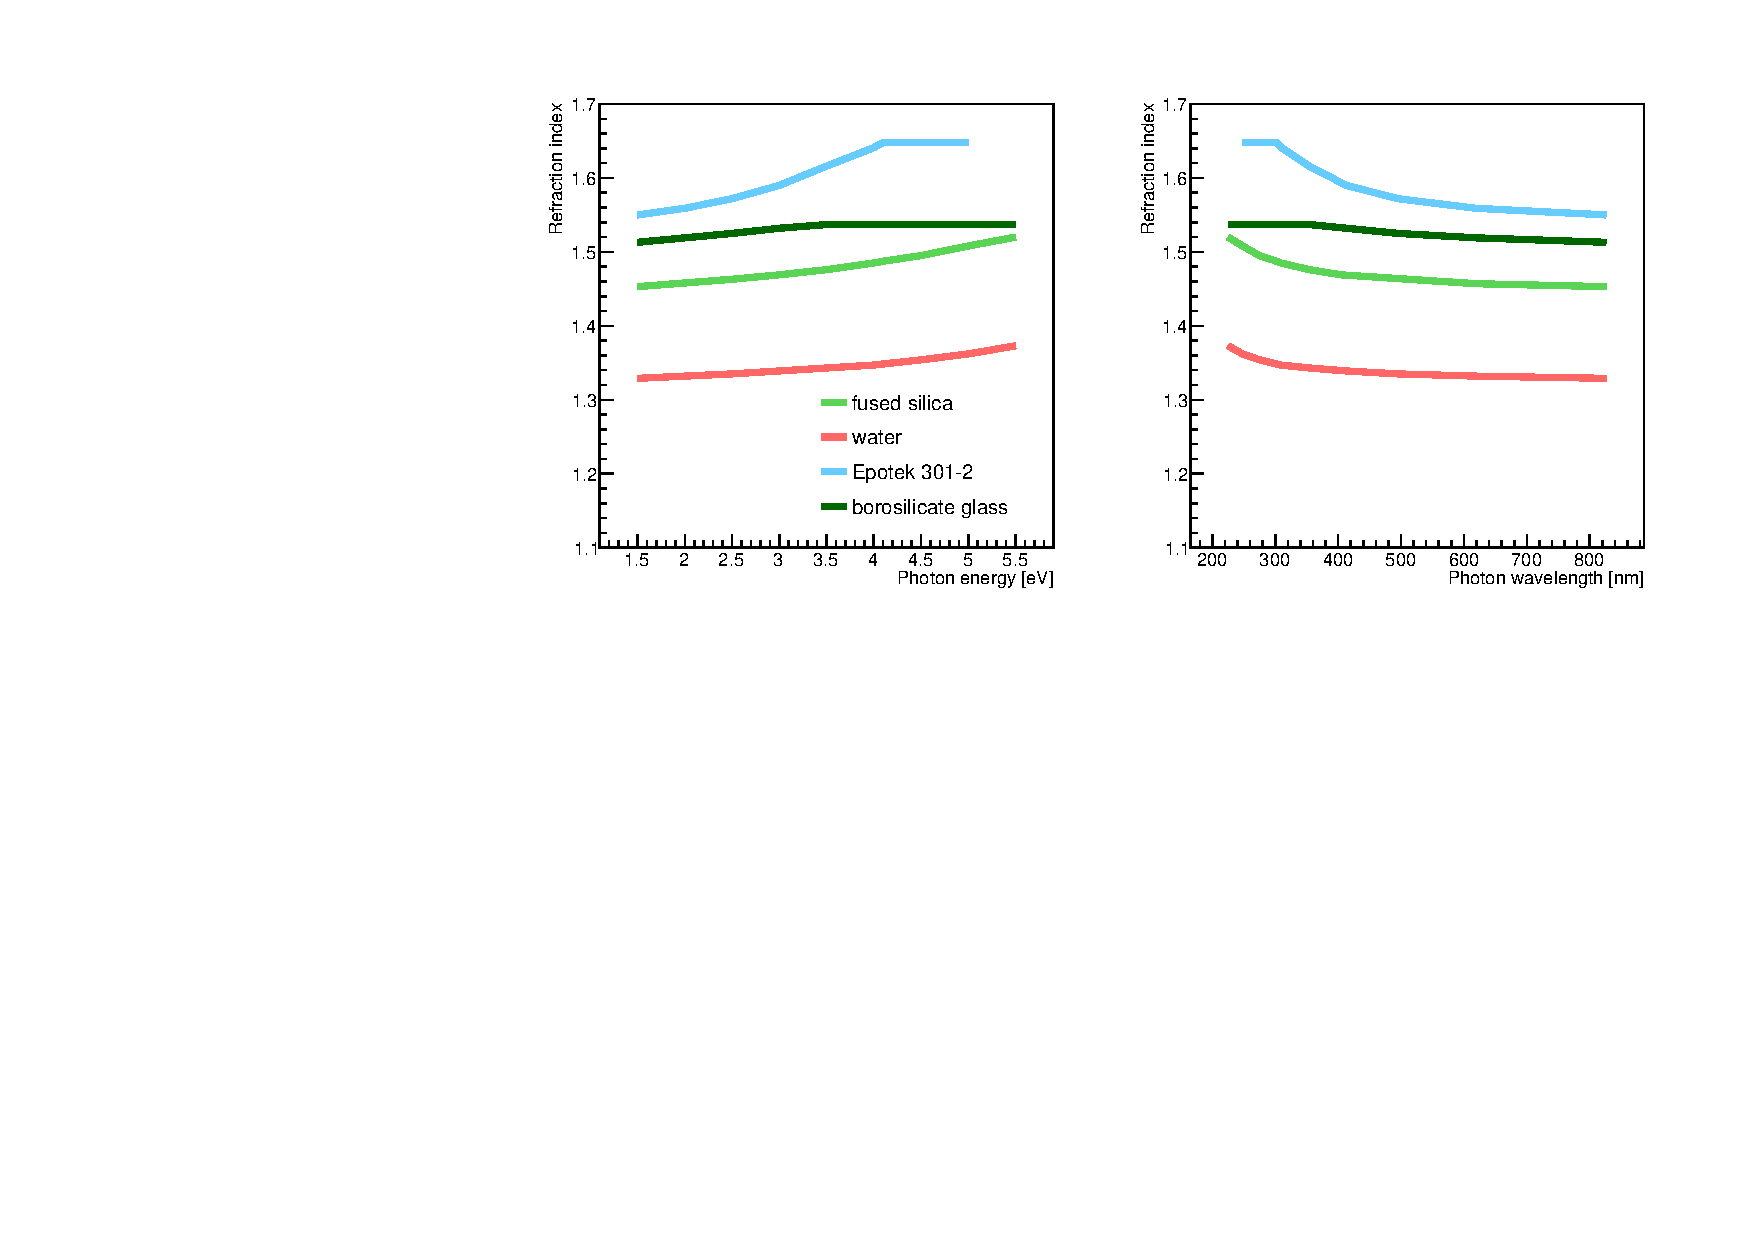
\includegraphics[angle=0,width=0.85\textwidth]{pics/refind1.pdf}
\caption{\label{pic:mat1}
Refraction index as a function of the photon energy (left) and wavelength (right) for the materials used in the simulation.
}
\end{figure}

\begin{figure}[!h]
\centering
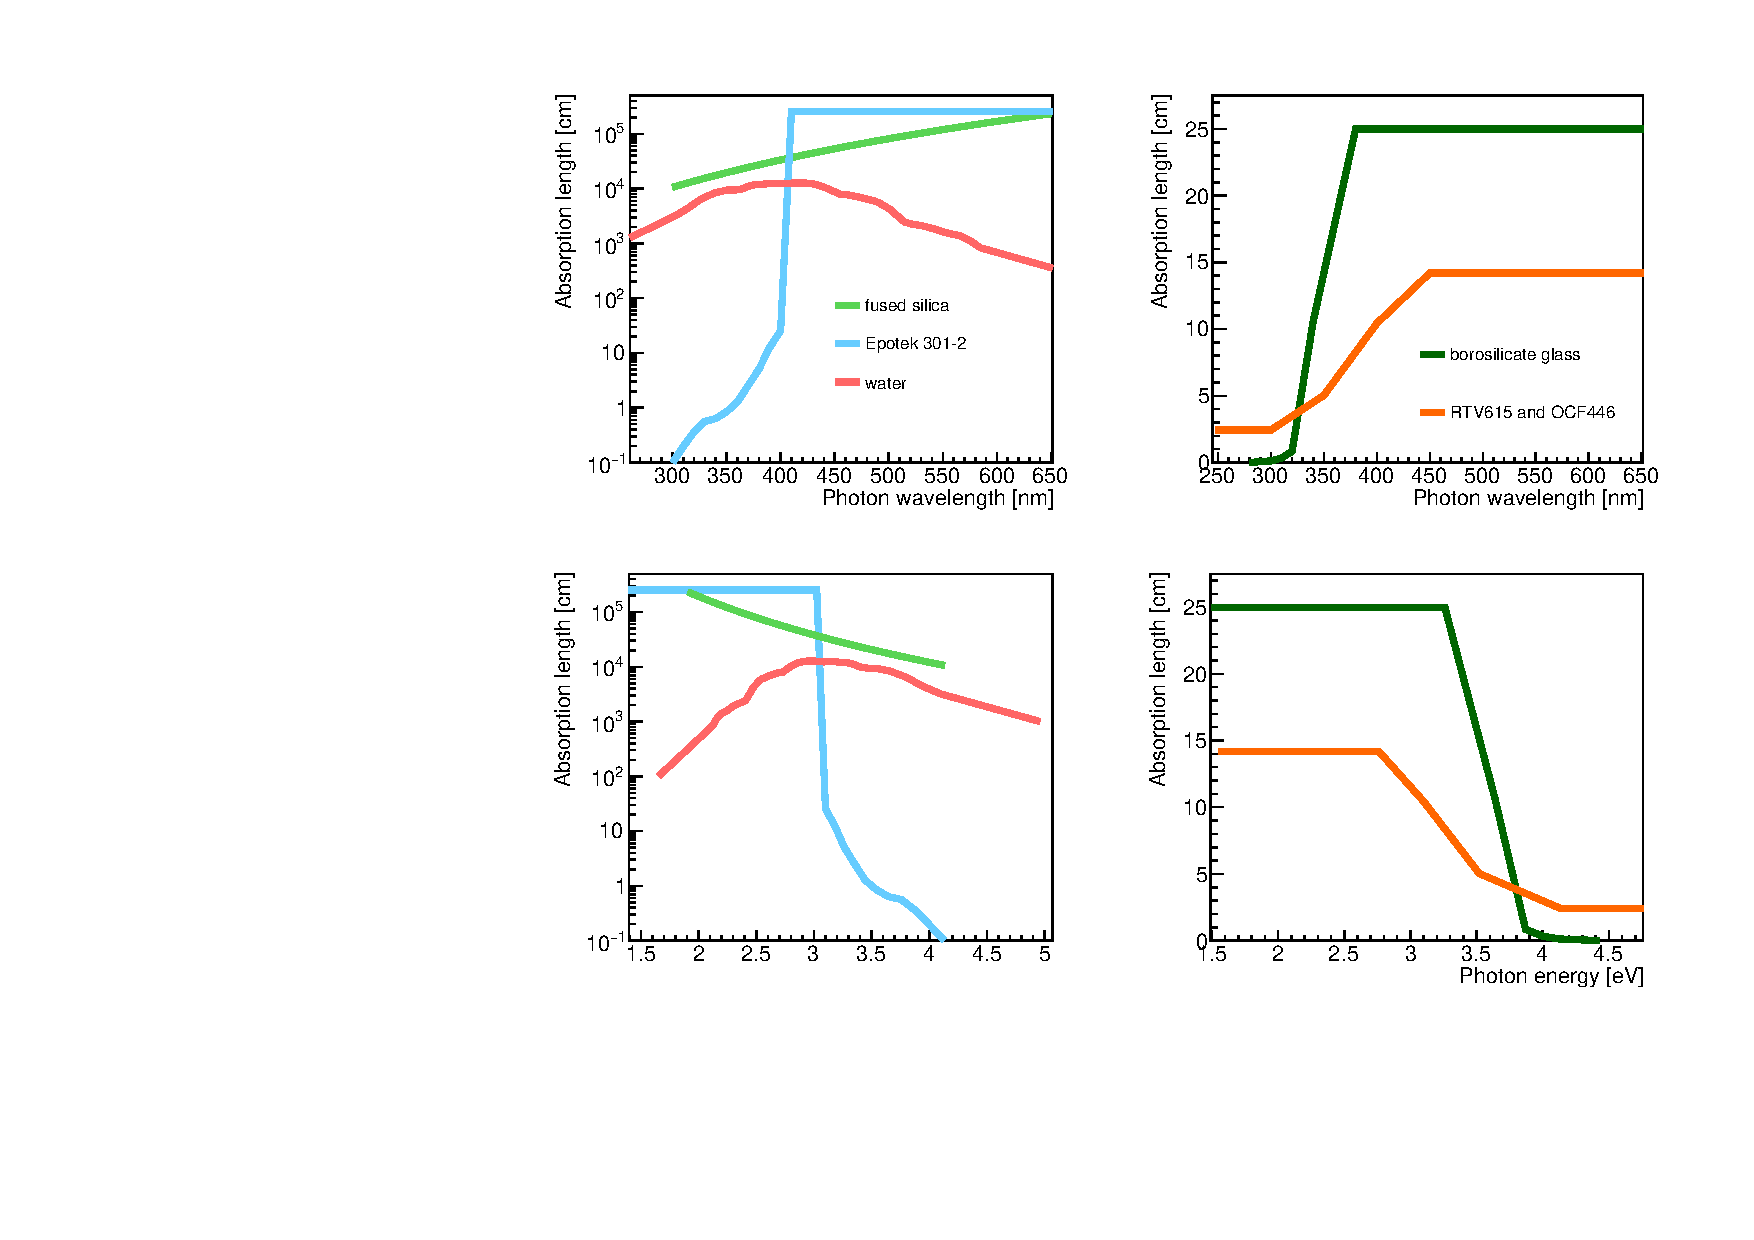
\includegraphics[angle=0,width=0.85\textwidth]{pics/ablen1.pdf}
\caption{\label{pic:mat2}
Absorption length as a function of the photon energy (left) and wavelength (right) for the materials used in the simulation.
}
\end{figure}

\subsubsection*{Epotek 301-2 optical glue}

The BABAR DIRC radiators are glued out of four pieces (see Fig.~\ref{pic:bar}) using Epotek $301-2$~\cite{Epotek} optical glue. The nominal thickness of the glue layer is $d_{glue} = 50 \mu m$. The same glue was used to attach the small wedge and the bar box window. The refraction index for Epotek 301-2 was taken from~\cite{EpotekData}. The absorption length was adopted from ??

\subsubsection*{Borosilicate glass}

H12700 PMTs can have either borosilicate glass or UV glass. The GlueX DIRC uses H12700 with borosilicate glass. The nominal thickness of the PMT window is $1.5$ mm (see specs sheet). The absorption length from the Schott Borosilicate Crown Glass data sheet is shown in Fig.~\ref{pic:gla}. The transmittance values should be corrected for Fresnel reflection. Fresnel reflection of the air-glass interface can be calculated as:

\begin{equation}
R = \Bigl( \frac{n_1 - n_2}{n_1 + n_2} \Bigr)^{2} = \Bigl( \frac{1.53 - 1}{1.53 + 1} \Bigr) ^{2} \approx 4.4\%,
\label{eq:fre}
\end{equation}

\noindent where $n_1 = 1.53$ is the refraction index for borosilicate glass, $n_2 = 1$ -- refraction index for air. The light passed the following tnerfaces: air-glass, glass-air. On each of two interfaces the Fresnel reflection should be taken into account leading to $R_{total} = 8.6\%$. The incident light was partly reflected ($R_{total}$), partly absorbed ($A$), and partly transmitted ($T$): $ R_{total} + T + A = 1$. For the absorption length $\lambda$ we need $1 - A = R_{total} + T = e^{-x/\lambda}$. 

\begin{figure}[htb]
\centering
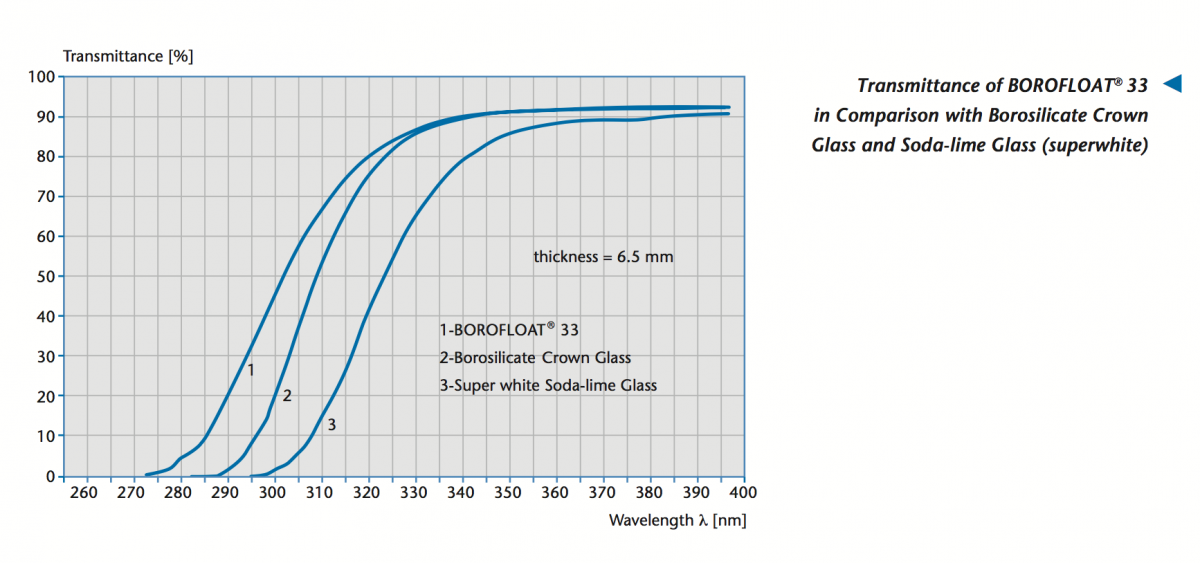
\includegraphics[angle=0,width=0.8\textwidth]{pics/glass.png}
\caption{\label{pic:gla}
Transmittance for the borosilicate glass (from the data sheet paper).
}
\end{figure}

\begin{equation}
\lambda = -x/\log(R_{total}+T) = -0.15/\log(0.086+T),
\label{eq:lam}
\end{equation}

\noindent here we assume glass thickness $x = 0.15$ cm. The following table shows absorption length for the borosilicate glass extracted from the Fig.~\ref{pic:gla} plot (line 2):

\begin{center}
\begin{tabular}{| c | c | c | c | c | c | c | c |}
\hline
wavelength [nm] & 280 & 300 & 310 & 320 & 340 & 380 \\
\hline
transmittance & 0 & 0.20 & 0.55 & 0.75 & 0.90 & 0.92 \\
\hline
$\lambda$ [cm] & 0 & 0.12 & 0.33 & 0.84 & 10.6 & 25.0 \\
\hline
\end{tabular}
\end{center}

\subsubsection*{Silicone cookies}

The material used to produce cookies is RTV615 by Momentive. The mixing ratio is $100 : 2.5$ (unlike the default mixing ratio of $10 : 1$), which makes the pad softer. The average thickness of the real cookies is $0.17$ cm, and the area is $5.2$ cm times $15.8$ cm. For the simulation the refraction index of the cookies is set constant $n = 1.406$, and the absorption length is taken from our measurements (see Fig.~\ref{pic:coo}). All the custom-made cookies have similar and good transmittance properties independently on the curing method or mixing ratio.

\begin{figure}[!tb]
\centering
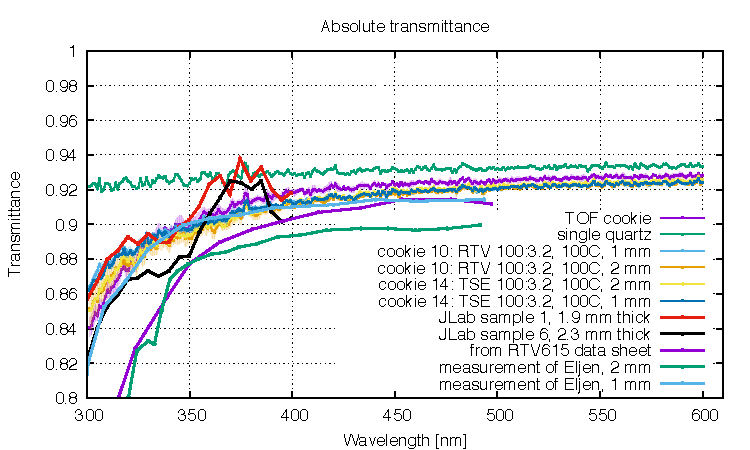
\includegraphics[angle=0,width=0.9\textwidth]{pics/transmittance1.pdf} \\
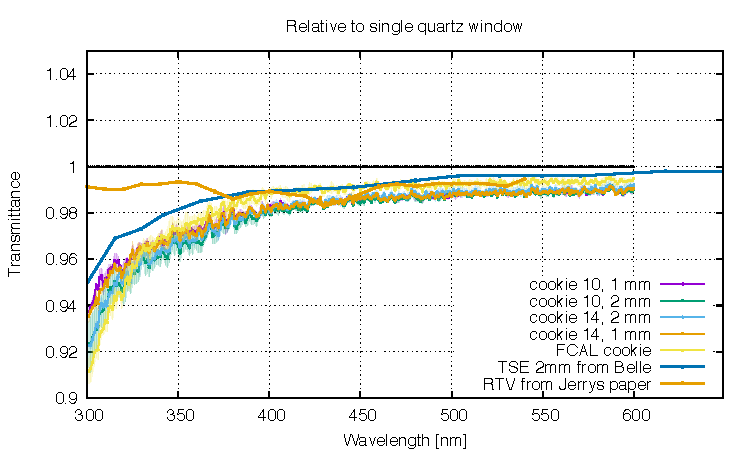
\includegraphics[angle=0,width=0.9\textwidth]{pics/cookie10_relQuartz.pdf}
\caption{\label{pic:coo}
Transmittance measurements for a set of custom-made silicone cookies. Absolute values (above), and relative to a single quartz window  (below). FCAL cookie is a pre-made cookie by Momentive (same RTV615 material, thickness $2$ mm). The data for TSE 2 mm cookie is taken from a plot on Belle II TOP cookies transmittance, which had poor resolution. The paper mentioned here is SLAC-PUB15942.
}
\end{figure}

The absorption length of the silicone was extracted from the absolute transmittance measurements (see Fig.~\ref{pic:coo} above). Transmittance was measured for the cookie sandwiched between two fused silica windows. Fresnel reflection of the air-fused silica interface can be calculated similarly to~(\ref{eq:fre}) using $n_1 = 1.47$ -- refraction index for fused silica leading to $R = 3.6 \%$. The total reflection loss for a single quartz window in air is then $R_{total} = 7.1 \%$. This estimation agrees with the absolute transmittance of quartz shown in Fig.~\ref{pic:coo} above (we can neglect the absorption inside the FS window). The absorption length for the silicone cookie can be calculated using~(\ref{eq:lam}), and we neglect the Fresnel reflections on the FS-cookie interface, which is about $R = 0.05 \%$.

%To extract absorption length for the silicone cookie, we have to account for the Fresnel reflections of the measured sample. Fresnel reflections on the FS-cookie interface is about $R = 0.05 \%$, so we neglect it. The incident light was partly reflected ($R$), partly absorbed ($A$), and partly transmitted ($T$): $ R_{total} + T + A = 1$. For the absorption lenght $\lambda$ we need $1-A = R_{total}+T = e^{-x/\lambda}$. 

%\begin{equation}
%\lambda = -x/\log(R_{total}+T) = -0.2/\log(0.071+T),
%\end{equation}

%\noindent here we assume cookie thickness of 2 mm. 
The following table shows absorption length for the silicone extracted from the Fig.~\ref{pic:coo} plot:


\begin{center}
\begin{tabular}{| c | c | c | c | c | c|}
\hline
wavelength [nm] & 300 & 350 & 400 & 450 & 600 \\
\hline
transmittance & 0.85 & 0.89 & 0.91 & 0.915 & 0.915 \\
\hline
$\lambda$ [cm] & 2.43 & 5.03 & 10.43 & 14.2 & 14.2 \\
\hline
\end{tabular}
\end{center}

\subsubsection*{Greasing silicone fluid OCF-446}

The Nye Lubricants OCF-446 silicone fluid is used to grease the cookies and, therefore, create a good optical coupling. The usage of particularly this product was inspired by the Belle II TOP experience. To introduce this material into simulation, its molecular structure is needed. OCF-446 is a vinyl terminated (diphenylsiloxane) dimethylsiloxane copolymer commonly referred to as a Phenyl Silicone. The molecular structure of this material is shown in Fig.~\ref{pic:ocf}. The diphenylsiloxane group in this schematic is repeated $m$ times, and dimethylsiloxane group -- $n$ times. In the material table (\texttt{hdds/Materials.xml}) the number of atoms of each type in one molecule is needed. I assume that $m = n = 1$, which leads to $20$ $C$ atoms, $30$ $H$ atoms, $4$ $Si$ atoms, and $3$ $O$ atoms. The data on the refraction index of OCF-446 is poor: there is only one measurement $n = 1.46$ at $\lambda = 589.3$ nm, which corresponds to photon energy of $\approx 2$  eV. No data on absorption length is available.

\begin{figure}[htb]
\centering
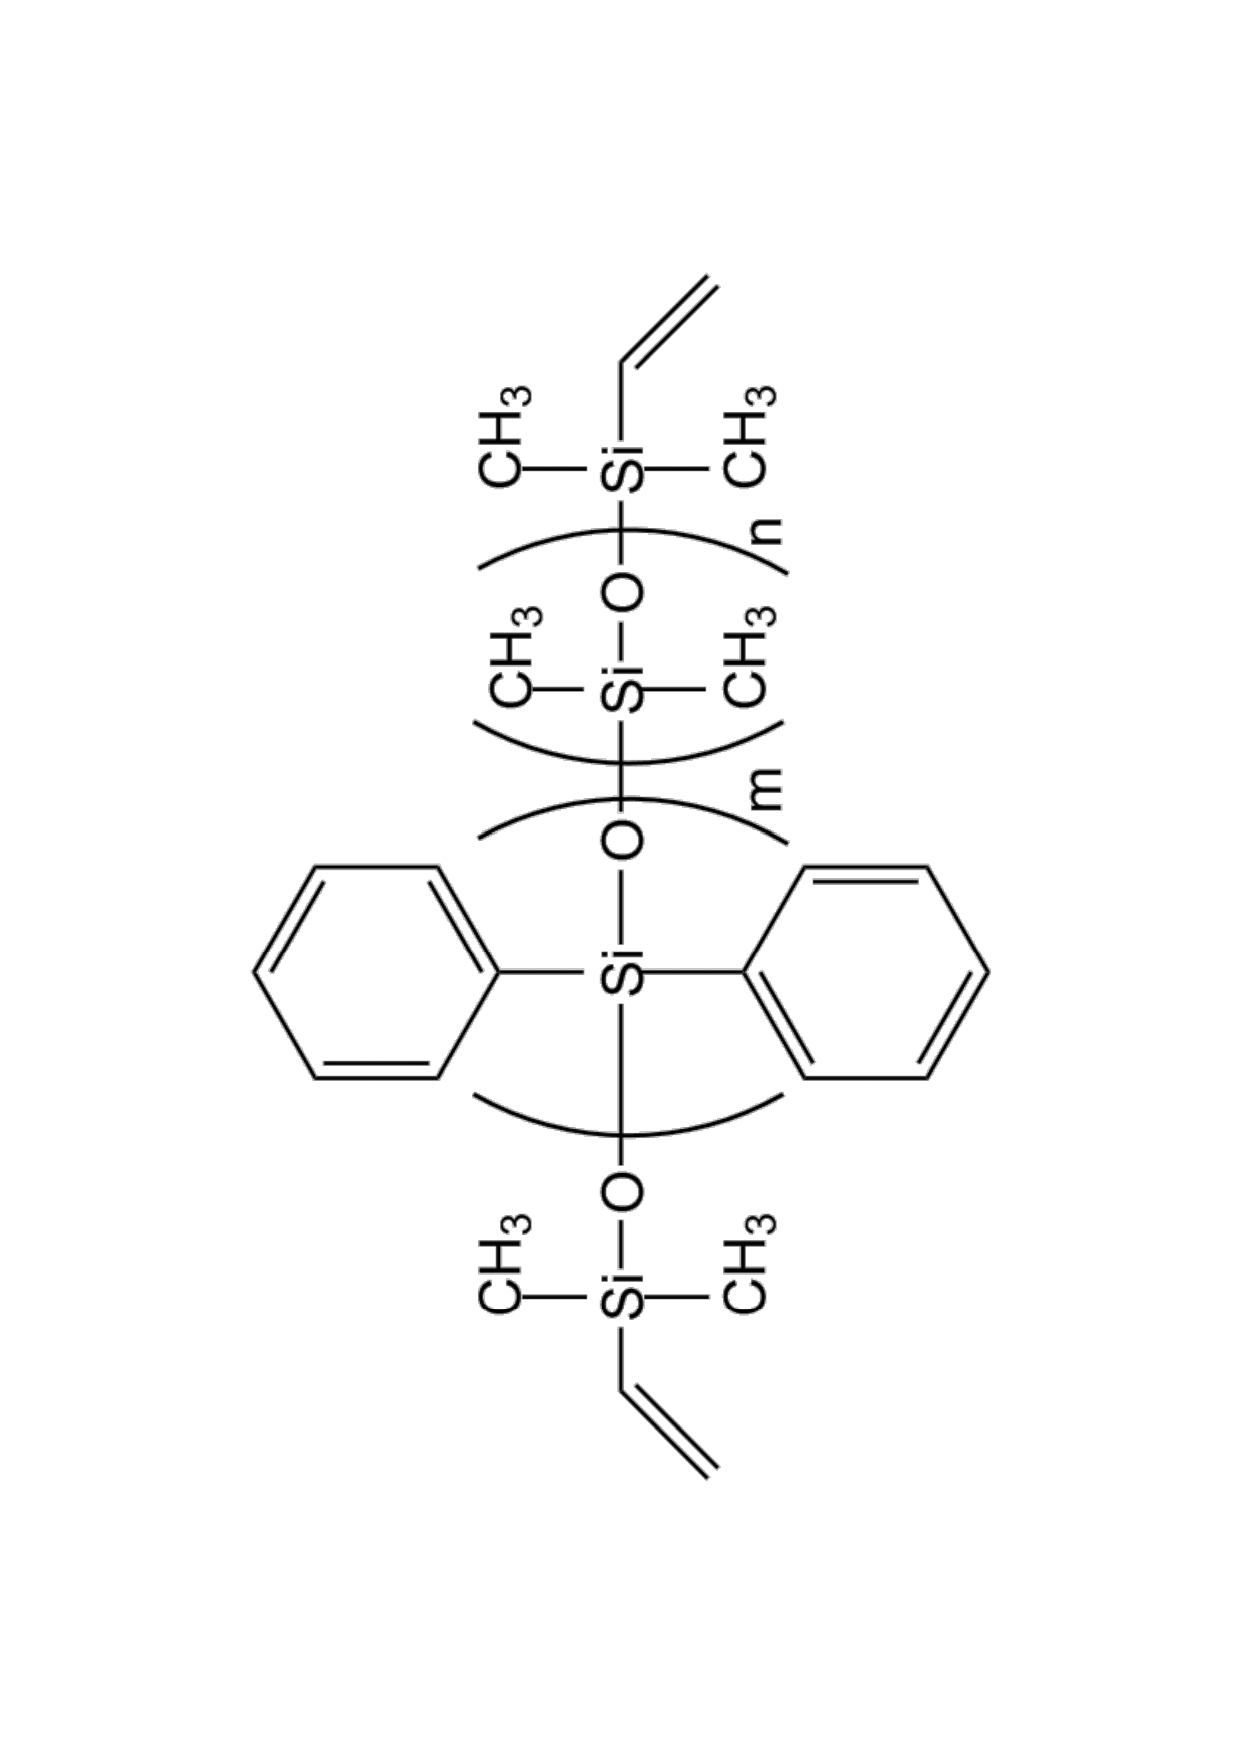
\includegraphics[angle=270,width=0.7\textwidth]{pics/ocf.pdf}
\caption{\label{pic:ocf}
A molecule of OCF-446 silicone fluid.
}
\end{figure}

There are two OCF-446 layers in the setup: one is between the PMT window and the cookie, another one is between the cookie and the window of the optical box. We can calculate the thickness of those layers based on the number of drops used. One drop is about $0.016$ g, density of the fluid is $1.04$ g/cm$^{3}$. Cookie area is $5.2$ cm times $15.8$ cm. I assume we use $2$ drops for the layer between the PMT and the cookie. This results into thickness of $0.0004$ cm. For the second layer we use $2$ drops to grease the cookie, and another $3$ drops to put in the middle of each PMT, which results into layer thickness of $0.00094$ cm. Both layers are introduced into the simulation, and there is no visible effect on the photon yield due to the greasing oil.

\subsubsection*{Bialkali photocathode}

According to Ref~\cite{pcpaper}, the photocathode is a thin layer of a multialkali (in our case bialkali) semiconducting alloy, which is evaporated onto the back side of the glass window during production. In the same paper we find, that it is quite difficult to extract properties of the photocathode itself. It can not be studied directly, as it is not chemically stable when exposed to air. Also, its properties might interefere with the birefringence, that is induced on the glass window by the mechanical stress due to the pressure difference (the interiour of the PMT is under vacuum). We use the simplified structure of the PMT: borosilicate window layer followed by a layer of photocathode with the thickness of $0.1$ cm (not realistic, but it does not matter, as our photons anyways get stopped in the photocathode). 

The quantum efficiency function defines properties of the photocathode, when the light is coming from air. For the case when instead of air we have a medium with $n > 1$ (we have the fused silica window with $n = 1.47$, in~\cite{pcpaper} they use scintillator with $n = 1.48$), the authors~\cite{pcpaper} state, that the effective quantum efficiency is slightly increased compared to the one stated in the data sheet. So in the simulation we will use the data sheet quantum efficiency as a conservative estimate. We use a refraction index of $n = 2.7$ to allow Geant4 performs reflection/refraction on the PMT window -- photocathode interface. We use a photocathode absorption length of $0.0001$ cm to stop Cherenkov photons in the photocathode volume.

%Geant4 needs absorption length $\lambda$ as the following:

%\begin{equation}
%I = I_{0} \cdot e^{-x/\lambda},
%\end{equation}

%\noindent where $I_{0}$ is the incident intensity, $I$ -- transmitted intensity, $x$ -- thickness of the sample. Transmittance $T = I/I_{0}$ for the photocathode $T = 1 - A$, where $A$ -- absorption. In the paper~\cite{pcpaper} we see $A$ (410 nm) $= 0.44$ and $A$ (440 nm) $=0.41$, we take $A = 0.42$ and calculate $\lambda$ based on this assumption and the photocathode thickness of $x = 0.1$ cm. We get absorption length of $\lambda = 0.184$ cm. The refraction index of photocathode is $2.7$~\cite{pcpaper}. 


